\documentclass[conference]{IEEEtran}
\usepackage{times}

% numbers option provides compact numerical references in the text. 
\usepackage[numbers]{natbib}
\usepackage{multicol}
\usepackage{amsmath} 
\usepackage{threeparttable}
\usepackage{booktabs}
\usepackage{graphicx}
\usepackage{subcaption}
\usepackage{threeparttable}
\usepackage{multirow}
\usepackage[dvipsnames]{xcolor}
\usepackage{cuted}
\usepackage{amsfonts}
\usepackage{tikz}
\usepackage{siunitx}
\setlength{\belowcaptionskip}{-5pt}
\usepackage[table]{xcolor}% http://ctan.org/pkg/xcolor

\DeclareCaptionLabelFormat{AppendixTables}{Appendix Table #2}
\usepackage{pifont}
\newcommand{\cmark}{\ding{51}}  % checkmark
\usepackage{caption}
\usepackage{pifont}
\usepackage[bookmarks=true]{hyperref}
\newcommand{\waglong}{Wiggle and Go!}
\newcommand{\wag}{WaG}
\newcommand{\adaptation}{\textit{adaptation model ($\Phi$)}}
\newcommand{\TODO}[1]{\textcolor{red}{#1}}


% after review, redefine as: \newcommand{\add}[1]{#1}
% \newcommand{\add}[1]{\textcolor{red}{#1}}

\newcommand{\JI}[1]{\textcolor{red}{[JI: #1]}}
\newcommand{\bart}[1]{\textcolor{blue}{[BD: #1]}}


\pdfinfo{
   /Author (Jakobsson, Mahajan, Pullalarevu, Suresh, Yao, Mao, Duisterhof, Syed, Ichnowski)
   /Title  (Wiggle and Go! System Identification for Zero-Shot Dynamic Rope Manipulation)
   /CreationDate (D:20101201120000)
   /Subject (Robots)
   /Keywords (Robots;Overlords)
}

\begin{document}

% paper title
\title{\waglong{} System Identification for Zero-Shot Dynamic Rope Manipulation}

% You will get a Paper-ID when submitting a pdf file to the conference system
% \author{Author Names Omitted for Anonymous Review. Paper-ID 806}

% You will get a Paper-ID when submitting a pdf file to the conference system
% \author{Author Names Omitted for Anonymous Review. Paper-ID 806}
\author{%
\authorblockN{%
Arthur Jakobsson$^1$,
Abhinav Mahajan$^1$,
Karthik Pullalarevu$^1$,
Krishna Suresh$^1$,
Yunchao Yao$^2$,
Yuemin Mao$^1$,\\
Bardienus Duisterhof$^1$,
Shahram Najam Syed$^1$,
Jeffrey Ichnowski$^1$ \\
}
\authorblockA{$^1$Robotics Institute, Carnegie Mellon University}
\authorblockA{$^2$The University of North Carolina at Chapel Hill}%
}
\maketitle
 
% Tighten the gap between the hero figure and the abstract.
% The `strip` environment (from cuted) leaves a large band of whitespace
% between \end{strip} and the two-column content that follows it. We
% neutralize the caption's own below-skip for this figure and add a
% negative \vspace after the strip to pull the abstract up.
\begin{strip}
    \centering
    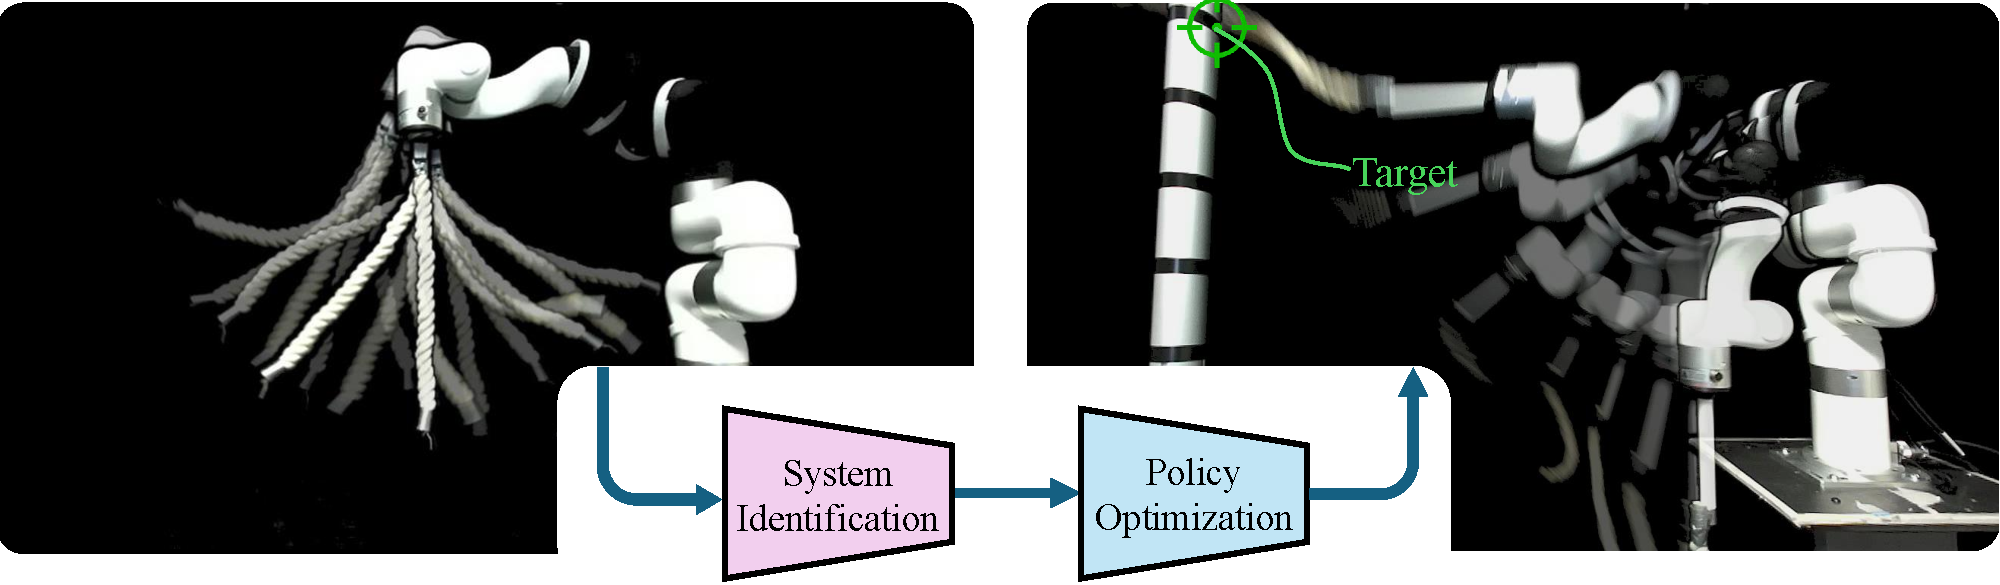
\includegraphics[width=1.95\columnwidth]{images/revised_hero2.pdf}
    \setlength{\abovecaptionskip}{4pt}%
    \setlength{\belowcaptionskip}{0pt}%
    \captionof{figure}{\waglong{} uses a brief \textit{wiggle} motion (left) to identify the dynamic behavior of a rope using a neural network model.
    This is fed into a goal-conditioned policy optimizer, which then \textit{goes!}, performing a dynamic fling (right), hitting the target in one shot. Our system identification model and policy optimizer work entirely in simulation enabling the wiggle and task rollout to be the only actions we perform in real.}
    \label{fig:system_overview}
\end{strip}
\vspace{-2em}
 

\begin{abstract}
Many robotic tasks are unforgiving; a single mistake in a dynamic throw can lead to unacceptable delays or unrecoverable failure. To mitigate this, we present a novel approach that leverages learned simulation priors to inform goal-conditioned dynamic manipulation of ropes for efficient and accurate task execution. Related methods for dynamic rope manipulation either require large real-world datasets to estimate rope behavior or the use of iterative improvements on attempts at the task for goal completion. We introduce Wiggle and Go!, a system-identification, two-stage framework that enables zero-shot task rope manipulation. The framework consists of a system identification module that observes rope movement to predict descriptive physical parameters, which then informs an optimization method for goal-conditioned action prediction for the robot to execute zero-shot in the real. Our method achieves strong performance across multiple dynamic manipulation tasks enabled by the same task-agnostic system identification module which offers seamless switching between different manipulation tasks, allowing a single model to support a diverse array of manipulation policies. We achieve a 3.55\,cm average accuracy on 3D target striking in real using rope system parameters in comparison to 15.34\,cm accuracy when our task model is not system-parameter-informed. We achieve a Pearson correlation coefficient of 0.95 between Fourier frequencies of the predicted and real ropes on an unseen trajectory. Project website: \normalsize\url{https://wiggleandgo.github.io/}
\end{abstract}

\IEEEpeerreviewmaketitle

\section{Introduction}
Before a sailor throws a mooring line or a climber flings a rope, they might instinctively give it a brief shake. This `wiggle' is not just a habit---it is a sophisticated probe. In that brief motion, the human nervous system assesses the rope's characteristics to calibrate for the subsequent throw to a perfect landing---because a failure can have disastrous consequences.
Robots performing similar dynamic tasks will be blind to these hidden dynamics, and if failures are unrecoverable (e.g., tangled, broken, or caught ropes) or lead to unacceptable delays, iteratively improving over multiple attempts may be too risky.
To bridge this gap, we propose a framework that replicates this intuitive human strategy: using a diagnostic probing action to decode an object's physical identity before committing to a high-stakes dynamic maneuver.

We propose \waglong{} (\wag{}), which features two primary steps (a) human-inspired system identification of ropes and (b) zero-shot goal-conditioned manipulation. Our observation and action rollout are pictured in Fig.~\ref{fig:system_overview}. Multiple prior works on dynamic rope manipulation explored the use of iterative refinement through an action policy~\cite{chi_iterative_2022, zhang_robots_2024}. Iteration serves as a strong prior for understanding the dynamics of the system but in some scenarios can be dangerous to the robot, surroundings, and the rope itself; therefore, we propose to understand rope dynamics through a short repeatable action or \emph{wiggle}.

Goal-conditioned rope manipulation poses a challenge for manipulation policies because of complex object properties and complex manipulator dynamics \cite{chi_iterative_2022}. Dynamic manipulation of ropes results in complex rapid movement. Therefore, we require a strong understanding of rope behavior in dynamic conditions to develop policies to handle such objects in real. With our system-identification method, we are able to understand dynamic motions of the rope in one context and predict the motion of the same rope in a different context.

Most dynamic rope manipulator methods also deal with the complexity of rope behavior modeling, either explicitly through physics simulations or indirectly by predicting the relationship between robot action and consequent rope movement. We do this explicitly by leveraging physics-based simulation and a parametrized representation of the rope to perform system identification (SysId).

\textit{We contribute a novel system identification method to act as a prior for goal-conditioned rope manipulation tasks.} Specifically, this paper contributes a method to perform system-identification on ropes by executing a safe action (``wiggle'') using a simple temporal convolutional neural network. Our system identification method is task-agnostic and therefore can be applied as a prior for a wide range of rope-manipulation tasks. Our SysId method demonstrates a high level of transferability between rope tasks and on a diverse range of ropes. Our experiments demonstrate our SysId-enabled, zero-shot manipulation method achieves a median 2.1\,cm accuracy in simulation and 3.55\,cm accuracy in real on 3D target striking (in comparison to our baseline 12.8\,cm and 15.29\,cm respectively for non-system-parameter-informed action), and achieves over 50\,\% success rate on complex multi-objective rope tasks like lobbing and draping. Across these qualitatively different manipulation primitives (dynamic target-striking, controlled lobbing, and draping) the same identification module supports every task without retraining. We demonstrate that the SysId-parameterized rope can predict rope behavior when transferred between dynamic tasks; and what types of wiggles are most informative for model training.


\section{Related Work}

\subsection{Rope Dynamics Through Data and Simulation}

Learning rope dynamics from large-scale data has been a persistent challenge due to the difficulty and safety concerns of collecting diverse real-world demonstrations. Early work by ~\citet{nair_combining_2017} required tens of thousands of autonomous interactions to learn rope dynamics from scratch. More recent self-supervised approaches ~\cite{wang2024selfsupervisedlearningdynamicplanar} reduce data requirements for dynamic cable manipulation but still rely on extensive autonomous interaction. Benchmark-driven methods like SoftGym ~\cite{lin2020softgym} provide standardized RL environments for deformable objects, while imitation learning approaches ~\cite{zhao2023learning, luo2024multistage} learn complex multi-stage behaviors from demonstration datasets. These data-intensive approaches achieve strong generalization but require extensive collection efforts that may be impractical for dynamic manipulation where failures can damage equipment or create safety hazards.

Sim-to-real transfer offers an alternative by training primarily in simulation. Domain randomization methods ~\cite{matas_simreal_2018, tiboni2023dropo} train policies across varied simulation parameters and lighting conditions to achieve transfer to real deformable objects, with recent work improving parameter distribution estimation from limited real data. Differentiable physics simulators \cite{hu2019chainqueen, jatavallabhula2021gradsim, chen2024deform, si2024difftactile} enable gradient-based parameter identification and trajectory optimization through backpropagation. Trajectory optimization frameworks \cite{jnadi2026scope, artinian2024optimal, yamakawa_simple_2012, yamakawa_dynamic_2013} leverage physics-based representations like Cosserat rods and convex formulations to generate smooth rope trajectories with explicit physics constraints. These simulation-based approaches provide strong inductive biases but often require either accurate prior parameters or extensive sim-to-real calibration.

\subsection{System Identification for Deformable Objects}

System identification approaches explicitly estimate physical parameters to bridge simulation and reality. Real2Sim2Real \cite{lim_planar_2022} optimizes simulator parameters to match observed trajectories for dynamic casting, though requiring extensive physical experiments for each new cable. GenORM \cite{kuroki_genorm_2025} and GenDOM \cite{kuroki_gendom_2025} condition policies on Young's modulus and Poisson's ratio estimated from point cloud observations during predefined lifting motions, demonstrating one-shot manipulation on single-stage planar tasks. \waglong{} differs in three key ways: (1) we use higher-dimensional, rope-specific parameters rather than material properties alone, \citet{lim_planar_2022} argues that Young's modulus-based simulation can create discrepancies for ropes with leads, (2) we demonstrate transferability across multiple complex 3D manipulation tasks rather than single-stage goals, and (3) we perform an analysis of how observation strategy (wiggle design) affects parameter prediction quality.

Recent work on learning-based dynamics models \cite{yang2022learning, wang2022offline} uses neural networks to capture rope behavior through recurrent architectures and graph representations. The hybrid offline-online approach by \citet{yu_shape_2022} combines simulation training with online adaptation, noting that model errors from changing object properties can necessitate refinement during manipulation. These learned dynamics approaches provide flexibility but typically predict implicit representations rather than interpretable simulation parameters. Our method learns to predict explicit rope parameters that can be used with standard physics-based trajectory optimization, enabling both interpretability and seamless integration with planning algorithms.

\subsection{Model Predictive Control and Dynamic Manipulation}

Model predictive control combines real-time optimization with feedback, offering robustness to modeling errors. Cable shaping MPC \cite{viljoen2024cable} combines learned interaction models with MPC for industrial routing, while aerial manipulation work \cite{sun2023nonlinear, sun2025agile} demonstrates aggressive cable-suspended load manipulation through nonlinear MPC accounting for full dynamics. These methods excel at online adaptation through continuous re-planning, though computational overhead typically limits them to slower quasi-static tasks. Our approach complements MPC methods by providing accurate parameter estimates that could improve their simulation models, while targeting the sub-second dynamic motions where pre-execution planning informed by system identification offers advantages over continuous re-optimization.


\begin{figure*} [t]
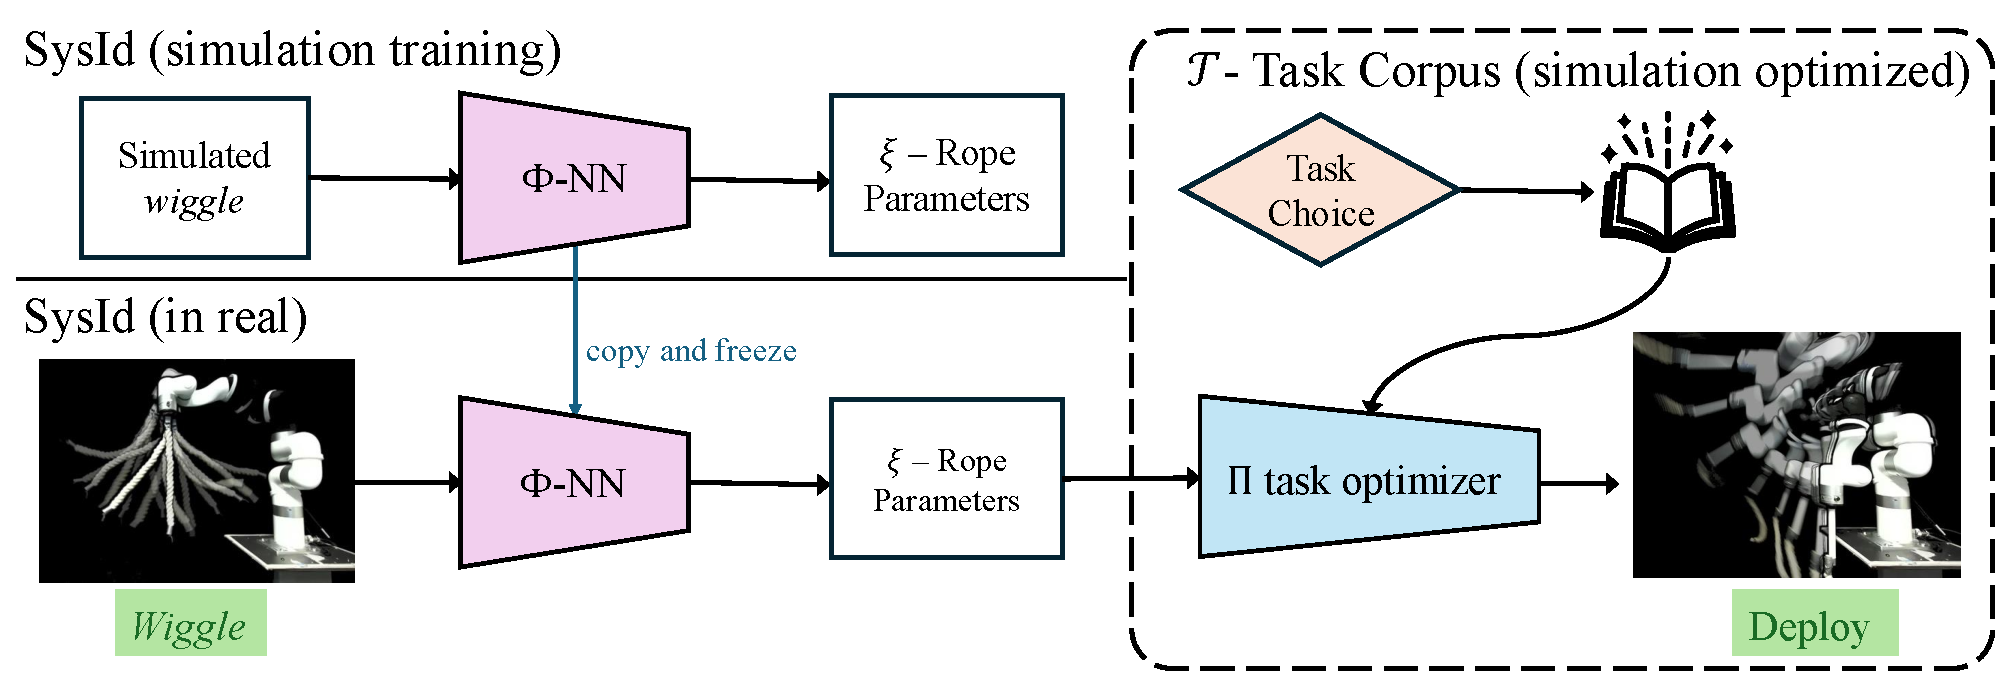
\includegraphics[width=2\columnwidth]{images/pipeline_figure2.pdf}
\caption{The \wag{} pipeline. We train a system identification neural network $\Phi$-NN entirely in simulation. We perform a wiggle in real as an input  for $\Phi$-NN. The output of these parameters are used to optimize an action for a chosen task which is then executed in real. Items highlighted in \textcolor{Green}{green} are the only elements of our procedure performed in real, once each.}\label{fig:pipeline}
\end{figure*}
\subsection{Iterative Learning Methods}

Iterative learning control refines policies through repeated trials \cite{bristow_survey_2006}. For dynamic rope manipulation, \citet{chi_iterative_2022, zhang_robots_2024} achieve strong results across diverse ropes and tasks through progressive refinement, typically requiring 5-10 trials per goal to achieve precise manipulation. Our method seeks to address scenarios where repeated attempts pose risks of rope damage, equipment failure, or environmental hazards. Critically different, our system identification module is task-agnostic so the same wiggle observation can support multiple downstream manipulation tasks, enabling seamless switching between different goals without additional real-world trials.


\subsection{Adaptation Through Privileged Learning}

Our adaptation approach draws inspiration from privileged learning frameworks like Rapid Motor Adaptation \cite{kumar_rma_2021, qi_-hand_2022, liang_rapid_2024}, which train policies with privileged environmental information in simulation while adaptation modules learn to infer hidden factors from observations. However, our implementation differs fundamentally: rather than implicit latent representations for online adaptation during task execution, we perform explicit parameter estimation offline through a safe observation action. This design enables task-agnostic system identification where the same adaptation module supports multiple downstream policies, and leverages the interpretability of physics-based simulation parameters for deformable object manipulation.
\section{Method}

\waglong{} has two stages: (1) a safe observation, a predefined \emph{wiggle} trajectory, excites rope dynamics for parameter estimation, and (2) task execution using trajectories optimized with these estimated parameters. Crucially, we decouple observation from task execution, enabling our task-agnostic system identification to support multiple manipulation tasks without retraining.

\wag{} observes rope motion through a wiggle trajectory to obtain visual features $\mathcal{O}$. The System Identification (SysId) model $\Phi: \mathcal{O} \rightarrow \Xi$ predicts rope system parameters $\xi \in \Xi$ (e.g., stiffness, damping, mass distribution, link count). Given a task goal $g \in \mathcal{G}$ (e.g., 3D target position) and rope parameters $\xi$, an action policy $\Pi: \Xi \times \mathcal{G} \rightarrow \mathcal{A}$ generates a robot trajectory $\vec{a} \in \mathcal{A}$. The complete pipeline is as follows: 
\begin{enumerate}
    \item execute wiggle on real rope
    \item $\Phi$ predicts $\hat{\xi}$ from observations
    \item $\Pi$ optimizes trajectory $\vec{a}$ given $\hat{\xi}$ and $g$
    \item execute trajectory
\end{enumerate}

We maintain a task corpus $\mathcal{T}$ of learned policies, each optimized for different manipulation tasks (e.g., target striking and lobbing). The shared input structure of $\mathcal{T}$ is enabled by the task-agnostic nature of our SysId model.
Figure~\ref{fig:pipeline} illustrates the complete system architecture.

\subsection{Action Policy Optimization $\Pi$} \label{sec:cmaes-traj}

Each task in the corpus requires a policy $\Pi_{\text{task}}: \Xi \times \mathcal{G} \rightarrow \mathcal{A}$ that maps rope parameters and goals to executable trajectories. 
To avoid real-world trial and error, we optimize trajectories in simulation using predicted rope parameters $\hat{\xi}$ from the adaptation model~(\ref{phi_NN}). 
We use Drake~\cite{drake} for high-fidelity rope simulation and accurate simulation with dynamic motions.
We employ data-efficient, derivative-free optimization that can discover effective trajectories within a few hundred simulations per rope-task pair.

\subsubsection*{Task Setup}
We choose three toy tasks to represent our task corpus: 3D point striking, lobbing, and draping shown in Figure~\ref{fig:drake_sim}. The lobbing task is motivated by controlled placement strategies in deformable object manipulation ~\cite{chen2022garment}. 3D point striking is the most complex to solve because it needs to minimize distance to a difficult-to-reach object; however, the other two tasks require more multi-objective optimization. Described fully in Section~\ref{sec:cmaes_traj}, both draping and lobbing have a more complex reward consisting of minimizing the distance of multiple points for draping and maintaining a position for draping. Our task setup (Figure~\ref{fig:drake_sim}) uses a UFactory xArm 7 robot manipulator~\cite{ufactory2022xarm7}. For all tasks, we attach ropes to a 20\,cm pole extender to increase the moment arm, the xArm's joint velocity limits require this leverage for dynamic motions like whipping. The target is positioned at the top of a vertical pole in the simulation. We track the rope tip (final link) position and minimize its 3D Euclidean distance to the target as our optimization objective. 


\begin{figure}[t]
    \centering
    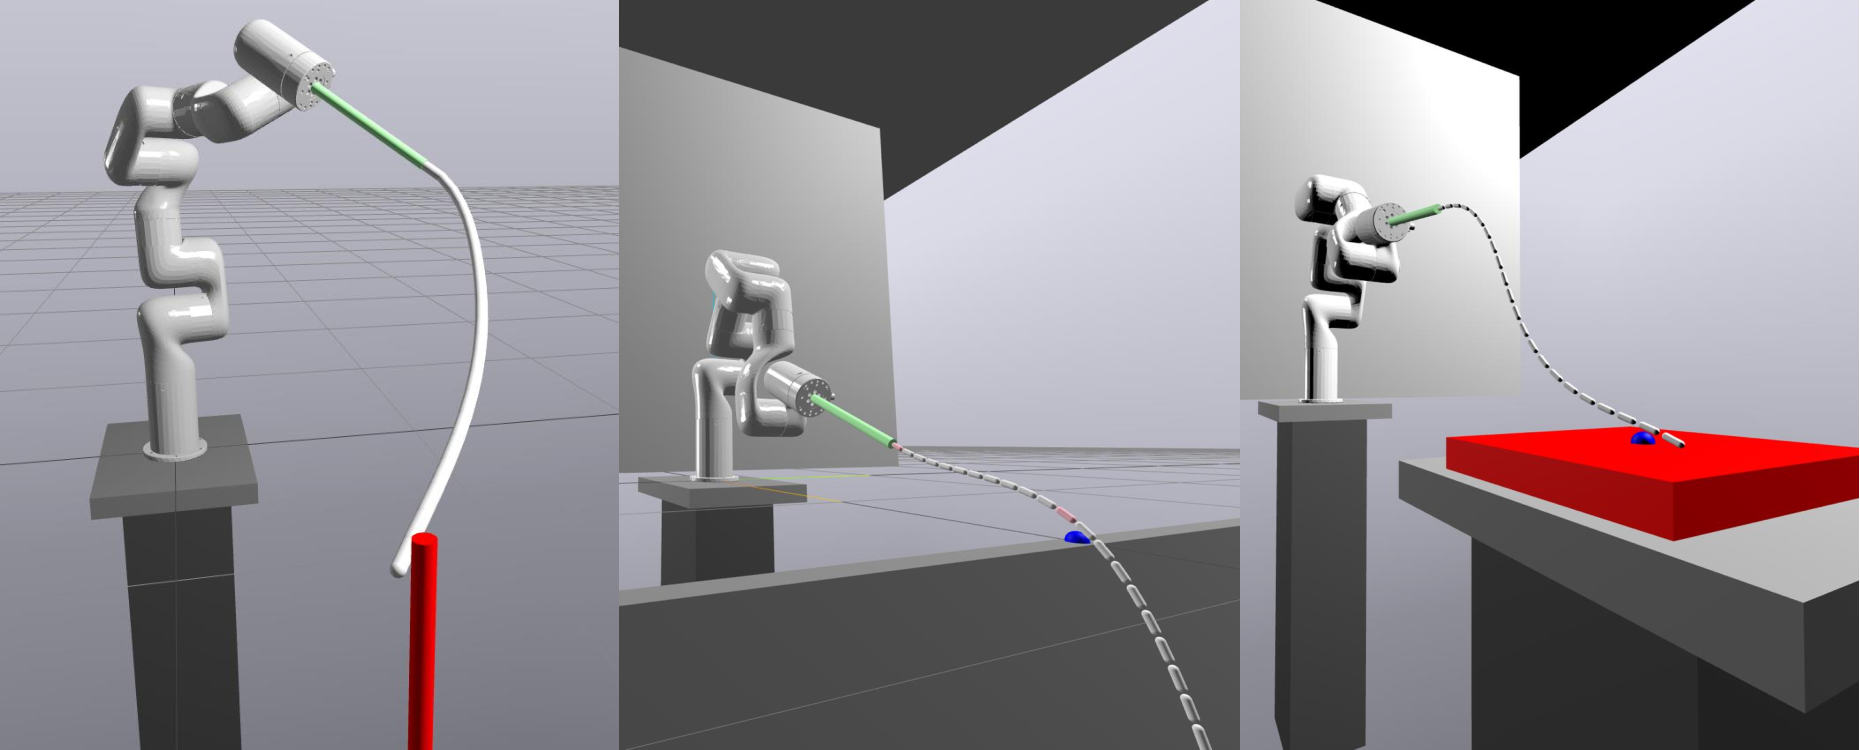
\includegraphics[width=\columnwidth]{images/drake_setups.pdf}
    \caption{Our task setups in Drake. \textcolor{SeaGreen}{Green:} rope extender for leverage. \textcolor{RedOrange}{Red:} target location is the top of the pole. \textcolor{Blue}{Blue:} targets locations}
    \label{fig:drake_sim}
\end{figure}

\subsubsection*{CMA-ES Trajectory Optimization}\label{sec:cmaes_traj}
We use Covariance Matrix Adaptation Evolution Strategy (CMA-ES)~\cite{cmaes}, a stochastic optimization algorithm that adapts its search distribution based on the success of sampled solutions. At each iteration, CMA-ES-traj (CMA-ES for trajectory optimization) samples a population of candidate trajectories from a multivariate Gaussian distribution, evaluates their fitness (task error in simulation), and updates the distribution's mean and covariance matrix to concentrate search around promising regions. This adaptive mechanism enables efficient exploration of the trajectory space without requiring gradient information from a hand-tuned reward function. We design a simple reward function for each of our three tasks. For 3D pole striking, we minimize distance of the tip location to the pole location; for lobbing, we employ a staggered reward function that first rewards the policy for nearing the target location and then we mix a reward for it to remain at that location, encouraging slow and controlled lobbing; finally, for draping, we employ a more complicated staggered reward that relies first on rewarding for the middle joint of the rope to near the top of the wall, for the tip to move forward and then finally for the tip to go to a lower point while the midpoint still targets the top of the wall. In all models, we also provide a penalty for any actions where the pole or rope nears unwanted regions such as the robot's base, the wall and ceiling. We additionally apply a heavy penalty for collisions between the robot and the rope or the extender pole. We did not observe robot self-collisions during optimization and so did not add an explicit self-collision penalty; one could be incorporated analogously to our existing joint-velocity constraint if a task required it. We found that these multifaceted reward structures provided the signal necessary for CMA-ES-traj to optimize and find successful trajectories. 

We parameterize trajectories using three sequential waypoints in the robot's joint space and interpolate between joint positions with a cubic spline to generate smooth, continuous joint trajectories subject to velocity constraints. This low-dimensional representation (21D parameters for a 7-DOF arm) significantly reduces the search space compared to direct optimization of full trajectories. For the more complex tasks, we limited exploration to planar actions where we only optimize the three joints that move in the plane of motion (9D parameters). Joint-space waypoints also avoid inverse kinematics singularities and naturally respect joint limits and velocity constraints, both critical for a controlled execution on physical hardware. For each rope parameter set $\xi$ and goal $g$, CMA-ES-traj runs for up to 25 iterations with 60 samples per iteration. The initial CMA-ES sampling distribution is unbiased for 3D pole-striking, in order to encourage broad exploration of the action space. For lobbing and draping, where the optimization landscape is more multi-modal, we bias the initial distribution toward a lifting motion which is a reliable warm start for both tasks that expedites convergence.


\subsubsection*{Simulation Setup and Implementation}
We represent ropes in simulation using the link, ball joint chains, following Lim et al.~\cite{lim_planar_2022}, where the rope is modeled as a series of rigid spheres connected by ball joints with stiffness $k$ and damping parameters $c$. Each link has an associated mass and radius for accurate inertial calculations. We vary the rope parameters across the ranges to match real ropes in household and industrial settings.  In experiments, we trained on parameters in the ranges in Table~\ref{tab:in_domain_results}. 
Following Lim et al.~\cite{lim_planar_2022}, we also include lead weights at the rope tip to model common real-world scenarios where ropes are used to cast or manipulate attached objects. The lead weight also increases the effective reach by providing momentum to the rope tip during dynamic motions.

The nine parameters we will estimate (Table~\ref{tab:in_domain_results}) are behavioral descriptors of this ball-joint representation rather than direct measurements of a physical rope: they describe the rope's dynamic response inside our simulator, and do not correspond one-to-one to measurable qualities of the ropes. We visually estimate that the training ranges we chose to span a wide behavioral distribution, and the in-distribution ropes in our real-world evaluation (Table~\ref{tab:rope_descriptions}) remain within this distribution from thin twine to stiff polyester that requires appreciable force to bend.

\subsection{Adaptation Model $\Phi$}\label{phi_NN}

Dynamic manipulation requires rope-specific trajectories; different ropes behave fundamentally differently based on their stiffness, mass distribution, and damping. We optimize trajectories in simulation (Section~\ref{sec:cmaes-traj}), but this requires knowing the rope's physical parameters. Real ropes lack specification sheets, so we infer parameters from observed behavior. Our safe wiggle is designed to excite rope dynamics through low-risk, repeatable motion, decoupling system identification from potentially dangerous task execution.

The mapping from dynamic rope motion to underlying physical parameters is complex and non-linear. Manually deriving such relationships is intractable. We therefore frame this as a supervised learning problem: train $\Phi$-NN ($\Phi$-neural network) to predict parameters from observed motion. Simulation is essential for generating training data because it provides ground truth parameter labels that are impossible to obtain from real ropes (since we cannot directly measure internal properties like stiffness or damping). We generate a diverse dataset of simulated ropes spanning the parameter ranges in Table~\ref{tab:in_domain_results}, each with known ground truth. Once trained on this data, $\Phi$-NN generalizes to new ropes. We integrate it into our pipeline by observing a wiggle ($\mathcal{O}$), estimating parameters ($\Phi(\mathcal{O}) \rightarrow\hat{\xi}$), and then using $\hat{\xi}$ for trajectory optimization.

\subsubsection{Observation Collection with Safe Action}\label{sec:howtowiggle}

We collect observations by executing a planar wiggle trajectory $\omega_{\text{wiggle}}$ that oscillates the rope with the robot end-effector. The wiggle is designed to excite key rope properties (stiffness, damping, inertia, etc.) through controlled acceleration while maintaining visibility for tracking. In our wiggle exploration section~(\ref{tab:wiggle_ablation}), we suggest that the specific wiggle trajectory is not critical; any motion that sufficiently excites rope dynamics performs comparably. We do not provide any theoretical guarantees on the safety of the wiggle action, but we use this terminology to suggest that a known, more controlled action is less likely to cause physical damage to surroundings and itself.

\begin{table*}[t]
\centering
\footnotesize
\caption{Wiggle Study: Mean Absolute Error across wiggle variants (1000 test samples). Ablations systematically vary wiggle parameters: Abl 1-3 use 20° amplitude at 0.5, 0.75, 1.0 Hz; Abl 4-6 use 30° amplitude at 0.5, 0.75, 1.0 Hz; Abl 7-8 use random predefined trajectories. Main is the primary wiggle (joint 6 oscillation of the xArm) used throughout all experiments. Color gradient indicates relative performance per parameter (green = best, red = worst).}
\label{tab:wiggle_ablation}
\resizebox{\textwidth}{!}{
\begin{tabular}{l|c|c|c|c|c|c|c|c|c}
\toprule
\textbf{Parameter} & \textbf{Abl 1} & \textbf{Abl 2} & \textbf{Abl 3} & \textbf{Abl 4} & \textbf{Abl 5} & \textbf{Abl 6} & \textbf{Abl 7} & \textbf{Abl 8} & \textbf{Main} \\
 & \scriptsize{20°, 0.5Hz} & \scriptsize{20°, 0.75Hz} & \scriptsize{20°, 1.0Hz} & \scriptsize{30°, 0.5Hz} & \scriptsize{30°, 0.75Hz} & \scriptsize{30°, 1.0Hz} & \scriptsize{Random 1} & \scriptsize{Random 2} & \scriptsize{Joint 6} \\
\midrule
Number of links & \cellcolor{green!40}0.122 & \cellcolor{green!30}0.127 & \cellcolor{yellow!30}0.225 & \cellcolor{yellow!20}0.205 & \cellcolor{yellow!20}0.206 & \cellcolor{orange!30}0.360 & \cellcolor{red!50}2.098 & \cellcolor{red!30}1.453 & \cellcolor{green!60}0.098 \\
Rope length (m) & \cellcolor{green!40}0.007 & \cellcolor{green!20}0.013 & \cellcolor{yellow!30}0.017 & \cellcolor{yellow!20}0.015 & \cellcolor{yellow!30}0.018 & \cellcolor{orange!20}0.022 & \cellcolor{red!50}0.057 & \cellcolor{red!30}0.028 & \cellcolor{green!60}0.006 \\
Ball damping (N·s/m) & \cellcolor{green!60}0.010 & \cellcolor{green!20}0.033 & \cellcolor{yellow!30}0.038 & \cellcolor{green!30}0.018 & \cellcolor{green!20}0.031 & \cellcolor{red!50}0.096 & \cellcolor{yellow!30}0.036 & \cellcolor{orange!30}0.040 & \cellcolor{green!60}0.010 \\
Rope radius (m) & \cellcolor{green!60}0.002 & \cellcolor{green!20}0.003 & \cellcolor{green!20}0.003 & \cellcolor{green!20}0.003 & \cellcolor{yellow!30}0.004 & \cellcolor{red!50}0.006 & \cellcolor{green!20}0.003 & \cellcolor{orange!30}0.004 & \cellcolor{green!60}0.002 \\
Mass per unit length (kg/m) & \cellcolor{green!60}0.006 & \cellcolor{green!20}0.010 & \cellcolor{green!20}0.010 & \cellcolor{yellow!30}0.013 & \cellcolor{yellow!20}0.012 & \cellcolor{orange!20}0.014 & \cellcolor{red!50}0.019 & \cellcolor{orange!30}0.014 & \cellcolor{green!40}0.007 \\
Link extra scale & \cellcolor{green!40}0.153 & \cellcolor{yellow!20}0.160 & \cellcolor{yellow!20}0.160 & \cellcolor{yellow!30}0.179 & \cellcolor{yellow!30}0.169 & \cellcolor{red!50}0.241 & \cellcolor{orange!30}0.205 & \cellcolor{red!30}0.208 & \cellcolor{green!60}0.152 \\
Lead mass (kg) & \cellcolor{green!60}0.005 & \cellcolor{yellow!20}0.011 & \cellcolor{yellow!30}0.014 & \cellcolor{green!30}0.008 & \cellcolor{yellow!20}0.011 & \cellcolor{orange!30}0.018 & \cellcolor{red!30}0.021 & \cellcolor{red!50}0.016 & \cellcolor{green!60}0.005 \\
Lead radius (m) & \cellcolor{green!20}0.008 & \cellcolor{green!20}0.008 & \cellcolor{green!20}0.008 & \cellcolor{green!20}0.008 & \cellcolor{green!20}0.008 & \cellcolor{green!20}0.008 & \cellcolor{green!60}0.007 & \cellcolor{green!20}0.008 & \cellcolor{green!20}0.008 \\
Ball stiffness (N/m) & \cellcolor{green!40}0.118 & \cellcolor{orange!30}0.257 & \cellcolor{red!30}0.258 & \cellcolor{yellow!30}0.224 & \cellcolor{yellow!30}0.244 & \cellcolor{orange!30}0.336 & \cellcolor{red!50}0.388 & \cellcolor{red!30}0.322 & \cellcolor{green!60}0.111 \\
\bottomrule
\end{tabular}}
\end{table*}

In simulation, for a rope with $N$ links, we extract 3D positions of the link centers $\{p_t^{(i)} \in \mathbb{R}^3\}_{i=1}^N$ at each timestep $t$. We project these to 2D image coordinates using a calibrated pinhole camera model. Since our wiggle is planar by design, depth information is largely redundant, the rope motion occurs primarily in the image plane and all links remain visible from a single fixed viewpoint. Our wiggle ablation study (Section~\ref{sec:wiggleablation}) demonstrates that various planar wiggles achieve comparable parameter estimation performance, suggesting that temporal dynamics from in-plane motion discriminate rope properties. While stereo setups with non-planar motion could potentially improve inference of damping and stiffness, the single-camera approach balances simplicity with empirically validated performance (Section~\ref{sec:fullpipeline}).

\textbf{Feature Engineering.} We normalize positions relative to the first link: $\tilde{p}_t^{(i)} = p_t^{(i)} - p_t^{(1)}$. This provides two benefits: (1) the first link is attached to the robot end-effector (effectively a fixed hinge), conveying minimal rope-specific information, and (2) normalization provides robustness to calibration shifts between simulation and deployment. We then compute angular features from normalized positions, including angles relative to the first link and their temporal derivatives (angular velocity and acceleration) using centered finite differences with Gaussian smoothing. While derivative features improve performance in simulation, they amplify noise in real-world tracking. For simulation training we include all features; for real-world deployment we use only position and angle features: $\mathcal{O} = \{\tilde{p}_t, \theta_t\}$. A useful consequence of this choice is that $\Phi$-NN never consumes raw pixels: appearance and texture variations between the real ropes and our simulation do not enter the model, and therefore do not contribute to the sim-to-real gap.

\subsubsection{Network Architecture and Sim-to-Real Training}

\textbf{Architecture and Training Strategy.} $\Phi$-NN consists of a temporal convolutional encoder followed by an MLP that maps observations to normalized rope parameters $\hat{\xi} \in [0,1]^9$ (Table~\ref{tab:in_domain_results}).

To bridge the sim-to-real gap, we apply domain randomization in three ways: (1) calibration noise perturbs camera position and lookat point, (2) tracking noise applies anisotropic, temporally-correlated noise mimicking segmentation errors, with higher longitudinal than lateral variance, and (3) trajectory padding randomly adds frames at trajectory start to simulate delayed recording. Additionally, we apply progressive curriculum masking during training to prevent overfitting to specific temporal windows. We mask random contiguous blocks of frames, increasing the number of masked blocks as training progresses, and apply beginning-biased masking to force the model to rely on end-of-motion dynamics.

\subsection{Real-World Deployment}

Our complete system is designed for real-world deployment on physical robots for ropes with unknown quantitative parameters. The deployment pipeline follows our two-stage methodology: (1) execute wiggle and extract visual observations, (2) $\Phi$-NN estimates rope parameters $\hat{\xi}$, (3) optimize trajectory using $\hat{\xi}$ in simulation, (4) execute trajectory on the robot, and (5) measure task performance. The key challenges are obtaining visual observations compatible with $\Phi$'s training data and accurately measuring task error in metric space.

\textbf{Wiggle Observation.} We use a ZED Mini 2i camera positioned to match the calibrated pinhole camera from simulation. For the first frame, we segment the rope using Grounding SAM~\cite{ren2024grounded}, apply color-based filtering for refinement, and fit a spline to the extracted rope mask to represent the rope centerline. We then compute the cumulative arc-length along this centerline and resample points at uniformly spaced distances to obtain 2D keypoints. Co-Tracker~\cite{karaev2410cotracker3} tracks these points across all wiggle frames. Tracked 2D positions are normalized relative to the first link and converted to angular features using the same pipeline as simulation. For real-world deployment, we use only position and angle features ($\tilde{p}_t$, $\theta_t$) to avoid noise amplification from temporal derivatives. Domain randomization during $\Phi$'s training (calibration noise, tracking noise) ensures robustness to real-world imperfections.

\textbf{Trajectory Execution and Evaluation.} After $\Phi$-NN predicts parameters ($\hat{\xi}$), we optimize a trajectory in Drake with CMA-ES as explained in ~\ref{sec:cmaes-traj} and execute it on the xArm 7. To measure task error, we track the rope endpoint and target using HSV-based color filtering in the camera feed. The ZED camera's depth estimates convert 2D detections to 3D metric coordinates, allowing us to compute the minimum distance between rope endpoint and target.


\section{Experiments and Results}

We perform a series of experiments to evaluate the efficacy of our adaptation model, the transferability of rope system parameters from one dynamic context to another, and the full-pipeline accuracy of our system-identification-enabled zero-shot manipulation optimization method. We perform our tests on a diverse range of ropes and a chain. The chain represents an out-of-distribution example of a rope-behaving object, though we note that ropes are more accurately represented as ball joints than chains which would be closer to an alternating hinge joint. We describe the five ropes in Table \ref{tab:rope_descriptions} and the ropes can be seen in Fig. \ref{fig:ropes}. Our contribution lies in the ability of our system identification method to reliably produce informative system parameters. Therefore, we directly test the conveyed information from the wiggles, the simulation precision, the transferability from one dynamic context to another of the predicted system parameters, and the importance of system identification for task roll-out in real. 



\begin{table}[t]
\centering
\caption{In-distribution parameter ranges and estimation accuracy. Left: training distribution bounds for each rope parameter. Right: prediction error on 1000 held-out test samples.}
\label{tab:in_domain_results}
\begin{tabular}{lccc|cc}
\toprule
& \multicolumn{3}{c}{\textbf{Parameter Range}} & \multicolumn{2}{c}{\textbf{Estimation Error}} \\
\cmidrule(lr){2-4} \cmidrule(l){5-6}
\textbf{Parameter} & \textbf{Min} & \textbf{Max} & \textbf{Units} & \textbf{MAE} & \textbf{Rel. Error (\%)} \\
\midrule
Number of links & 20 & 26 & --- & 0.098 & 0.44 \\
Rope length & 0.45 & 0.65 & m & 0.006 & 1.13 \\
Ball damping & 0.001 & 0.05 & N·s/m & 0.010 & 33.73 \\
Ball stiffness & 0.05 & 1.0 & N/m & 0.111 & 33.82 \\
Rope radius & 0.003 & 0.015 & m & 0.002 & 36.37 \\
Mass per unit len & 0.02 & 0.12 & kg/m & 0.007 & 62.56 \\
Lead mass & 0.02 & 0.12 & kg & 0.005 & 45.2 \\
Lead radius & 0.015 & 0.045 & m & 0.008 & 28.81 \\
Link extra scale & 50 & 120 & \% & 0.152 & 19.85 \\
\midrule
\multicolumn{4}{l|}{\textbf{Overall}} & \textbf{0.045} & \textbf{30.7} \\
\bottomrule
\end{tabular}
\end{table}

\begin{figure} 
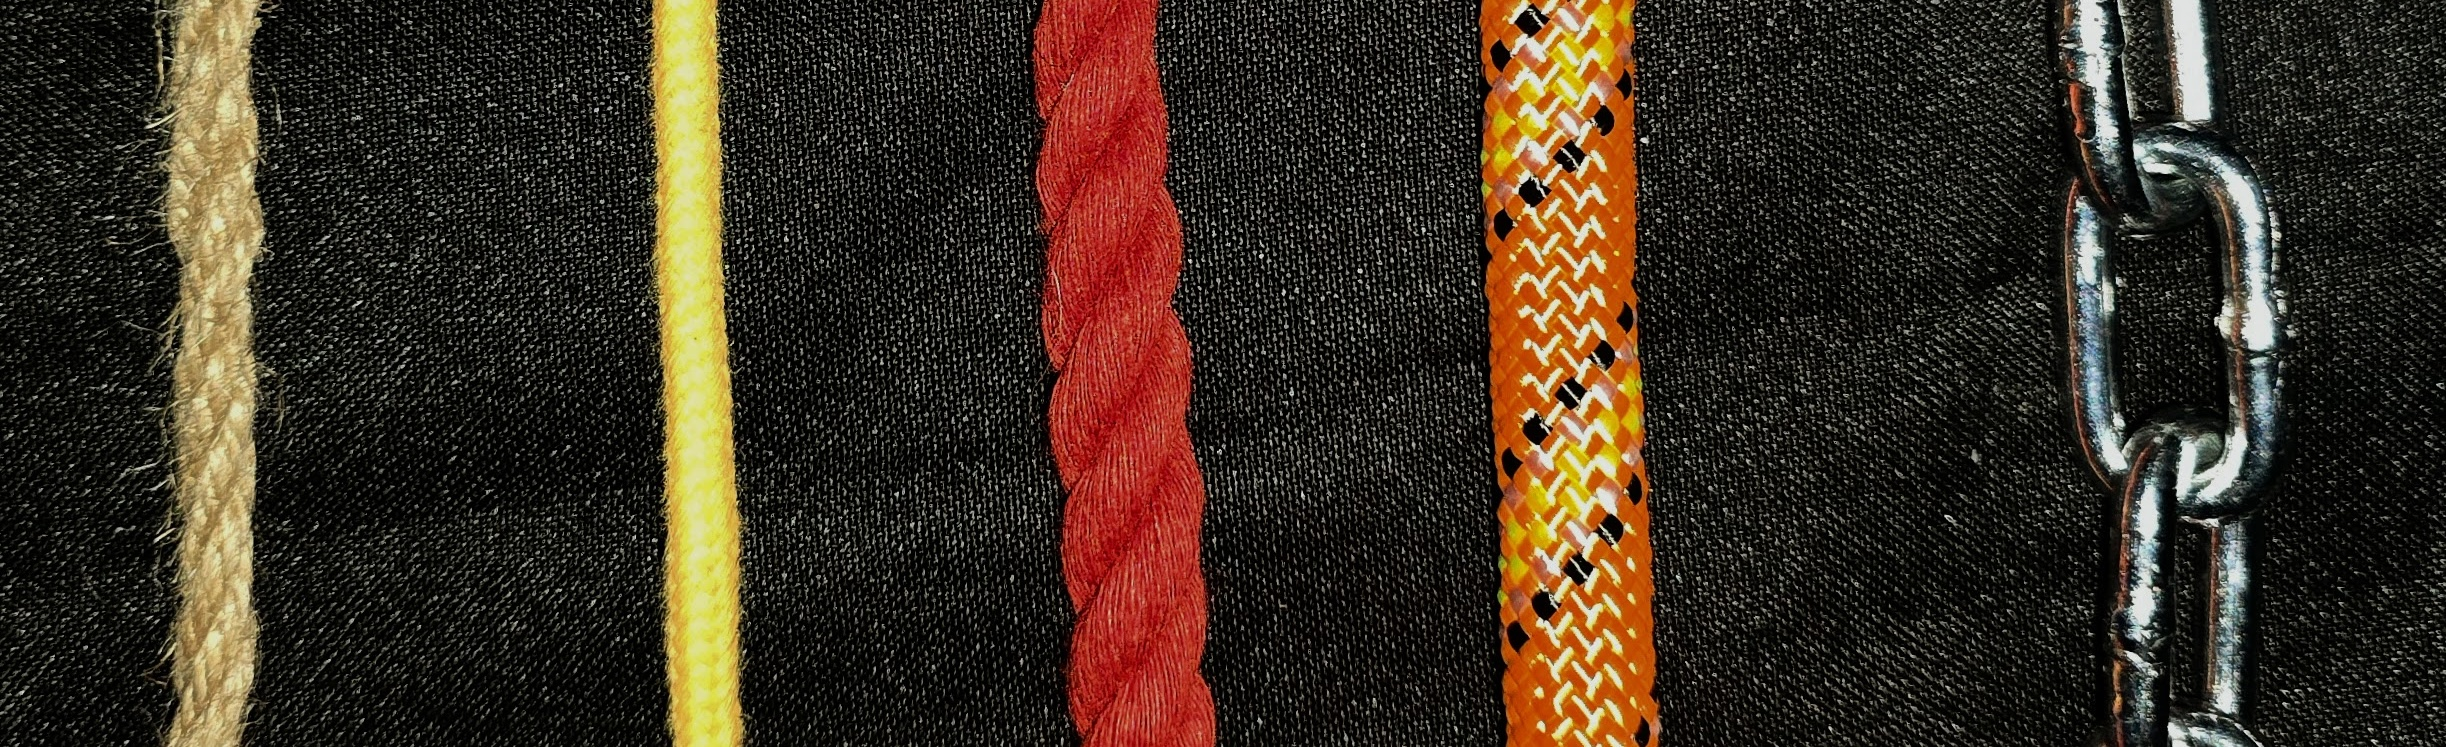
\includegraphics[width=\columnwidth]{images/ropes_narrow.jpg}
\caption{Five ropes types used in experiments. In order: \textcolor{Brown}{Brown}, \textcolor{Dandelion}{Yellow}, \textcolor{Red}{Red}, \textcolor{Orange}{Orange}, and \textcolor{CadetBlue}{Chain}.}\label{fig:ropes}
\end{figure}


\begin{table}[t]
\centering
\caption{Estimation of parameters, material, and physical description of test ropes}
\label{tab:rope_descriptions}
\begin{tabular}{lccccc}
\toprule
\textbf{Rope} & \textbf{Material} & \textbf{Stiffness} & \textbf{Damping} & \textbf{Weight} & \textbf{Radius} \\
& & & & \textbf{(kg/m)} & \textbf{(mm)} \\
\midrule
\textcolor{Brown}{Brown} & Twine & Slack & Low & 0.013 & 6 \\
\textcolor{Dandelion}{Yellow} & Cotton & Stiff & Medium & 0.011 & 5 \\
\textcolor{Red}{Red} & Cotton & Slack & Low & 0.033 & 9.5\\
\textcolor{Orange}{Orange} & Polyester & Stiff & High & 0.082 & 12.7\\
\textcolor{CadetBlue}{Chain} & Steel & Slack & Low & 0.52 & 4.8$\times$18\\
\bottomrule
\end{tabular}
\end{table}

\subsection{Adaptation Model Evaluation}

We evaluate $\Phi$-NN on three criteria: parameter estimation accuracy, robustness to distribution shift, and transferability to downstream tasks. All experiments use the model trained on 9000 simulated ropes with domain randomization enabled.

\subsubsection{Parameter Estimation Accuracy and Robustness}

\textbf{In-Domain Performance.} On 1000 test samples in simulation, $\Phi$-NN achieves 30.7\% aggregate relative error across all 9 parameters (Table~\ref{tab:in_domain_results}). The model accurately estimates geometric properties (rope length, number of links) with errors below 1.1\%. Inertial and damping properties observable only through dynamic motion prove more challenging, with mass per unit length showing the highest error. Stiffness, radius, and lead parameters fall in the mid-range. This distribution reflects the fundamental challenge of inferring mass distribution and damping from 2D projected motion. Note that relative errors are inflated for parameters with small absolute ranges, for instance, predicting mass per unit length as 0.0016 kg/m versus 0.001 kg/m yields 60\% relative error, yet these values produce similar rope behavior and can be compensated by other parameters due to multicollinearity in the physical model.


\textbf{Out-of-Distribution Robustness.} We test generalization by extending 4 parameters beyond training bounds: ball damping $\in [0.1, 1.5]$, mass per unit length $\in [0.05, 0.08]$, lead mass $\in [0.05, 0.2]$, and ball stiffness $\in [1.0, 1.5]$. On 1000 new test samples with 1-4 OOD parameters, the model exhibits stable relative error at 45-46\%, compared to 30.7\% in-domain. However, all OOD parameters show 100\% saturation, the model clamps predictions to training bounds rather than extrapolating. For example, ball damping predictions saturate at [0.016, 0.089] when targets span [0.100, 1.499]. This reflects a fundamental limitation: neural networks trained on bounded distributions cannot reliably extrapolate beyond observed ranges. While this limits applicability to ropes with drastically different properties, downstream trajectory optimization can compensate for bounded parameter errors more easily than unbounded extrapolations, and the saturated predictions still provide useful initialization compared to random sampling (Section~\ref{sec:fullpipeline}).

\textbf{Observation Robustness.} \label{sec:wiggleablation}We train 8 additional models using different planar wiggles: 6 systematically varying amplitude (20°, 30°) and frequency (0.5-1.0 Hz), and 2 random trajectories (Table~\ref{tab:wiggle_ablation}). The main wiggle achieves best overall performance, with Ablation 1 (20°, 0.5 Hz) close behind. Performance remains consistent across planar wiggles that sufficiently excite rope dynamics, no single wiggle dominates all parameters. Random trajectories (Ablations 7-8) show degraded performance on complex parameters. This validates our design principle: planar wiggles with adequate excitation enable accurate parameter inference regardless of specific trajectory. We hypothesize that stereo setups with depth cameras with non-planar motion could further improve inference of certain parameters like damping and stiffness.



\subsubsection{Transferability to Downstream Tasks}

Parameter-wise accuracy alone is insufficient, predicted parameters must work together to enable task execution. We validate transferability through motion fidelity (whether predicted parameters reproduce rope dynamics under different motions) and task-level performance (whether they enable effective trajectory optimization).

\textbf{Baseline: $\Phi$-CMAES.} To benchmark $\Phi$-NN, we implement an optimization-based baseline that directly fits simulation parameters to observed motion. Given a real wiggle trajectory (2D tracked points over time), $\Phi$-CMAES runs CMA-ES optimization to search the parameter space. Each iteration samples candidate parameter sets, simulates the wiggle in Drake with those parameters, projects the simulated 3D rope to 2D, and minimizes pixel-wise distance to the real trajectory (plus joint angle and velocity terms to aid convergence). We run 60 samples per iteration for 50 iterations. Unlike $\Phi$-NN, which relies on learned priors from training data, $\Phi$-CMAES performs brute-force parameter search without assumptions about rope behavior, thereby intentionally overfitting the rope to the wiggle. This makes it slower (3000 simulations vs. one forward pass) but potentially more robust to objects with dynamics far outside the training distribution, e.g., chains, where rigid dynamics differ significantly from flexible ropes. $\Phi$-NN's learned priors help it generalize across typical ropes but may hinder performance on fundamentally different deformable objects.

\textbf{Motion Fidelity.} We test whether predicted parameters capture rope dynamics beyond static accuracy. For 10 real ropes (5 types with 10g and 30g leads), we predict parameters from wiggle A, simulate a different wiggle B with those parameters, perform the same wiggle B with the real rope, and compare via Fourier frequency analysis and point-wise trajectory matching (Fig.~\ref{fig:pointwise-comparison}, Fig.~\ref{fig:fourier}, Appendix table 1). Both $\Phi$-NN and $\Phi$-CMAES achieve 0.95 average frequency correlation (Pearson correlation coefficient to measure linear correlation between the real and simulated frequencies), capturing dominant motion characteristics. 
$\Phi$-NN achieves 5.4\,cm/frame average error versus 5.8\,cm/frame for $\Phi$-CMAES, both substantially outperforming random parameters (13.6\,cm/frame).
Notably, $\Phi$-CMAES performs better on the chain (0.99 vs. 0.78 correlation), whose dynamic behavior differs significantly from rope training data distribution, demonstrating when optimization-based fitting is preferable. However, $\Phi$-NN generalizes reliably across typical rope variations without per-rope re-optimization.

Taken together, these two metrics characterize fidelity across the full trajectory, not only at its endpoint: Fourier correlation tracks whether the dominant oscillatory content of the motion is reproduced, while per-frame point distance measures spatial agreement at every timestep of the unseen motion. The $\sim$2.5$\times$ gap in per-frame error between $\Phi$-NN (5.4\,cm/frame) and random parameters (13.6\,cm/frame), combined with the 0.95 Fourier correlation, indicates that the parameters inferred from the wiggle reproduce the rope's dynamics throughout the trajectory, and generalize to motions $\Phi$-NN has never observed.


\begin{figure}[t]
    \centering
    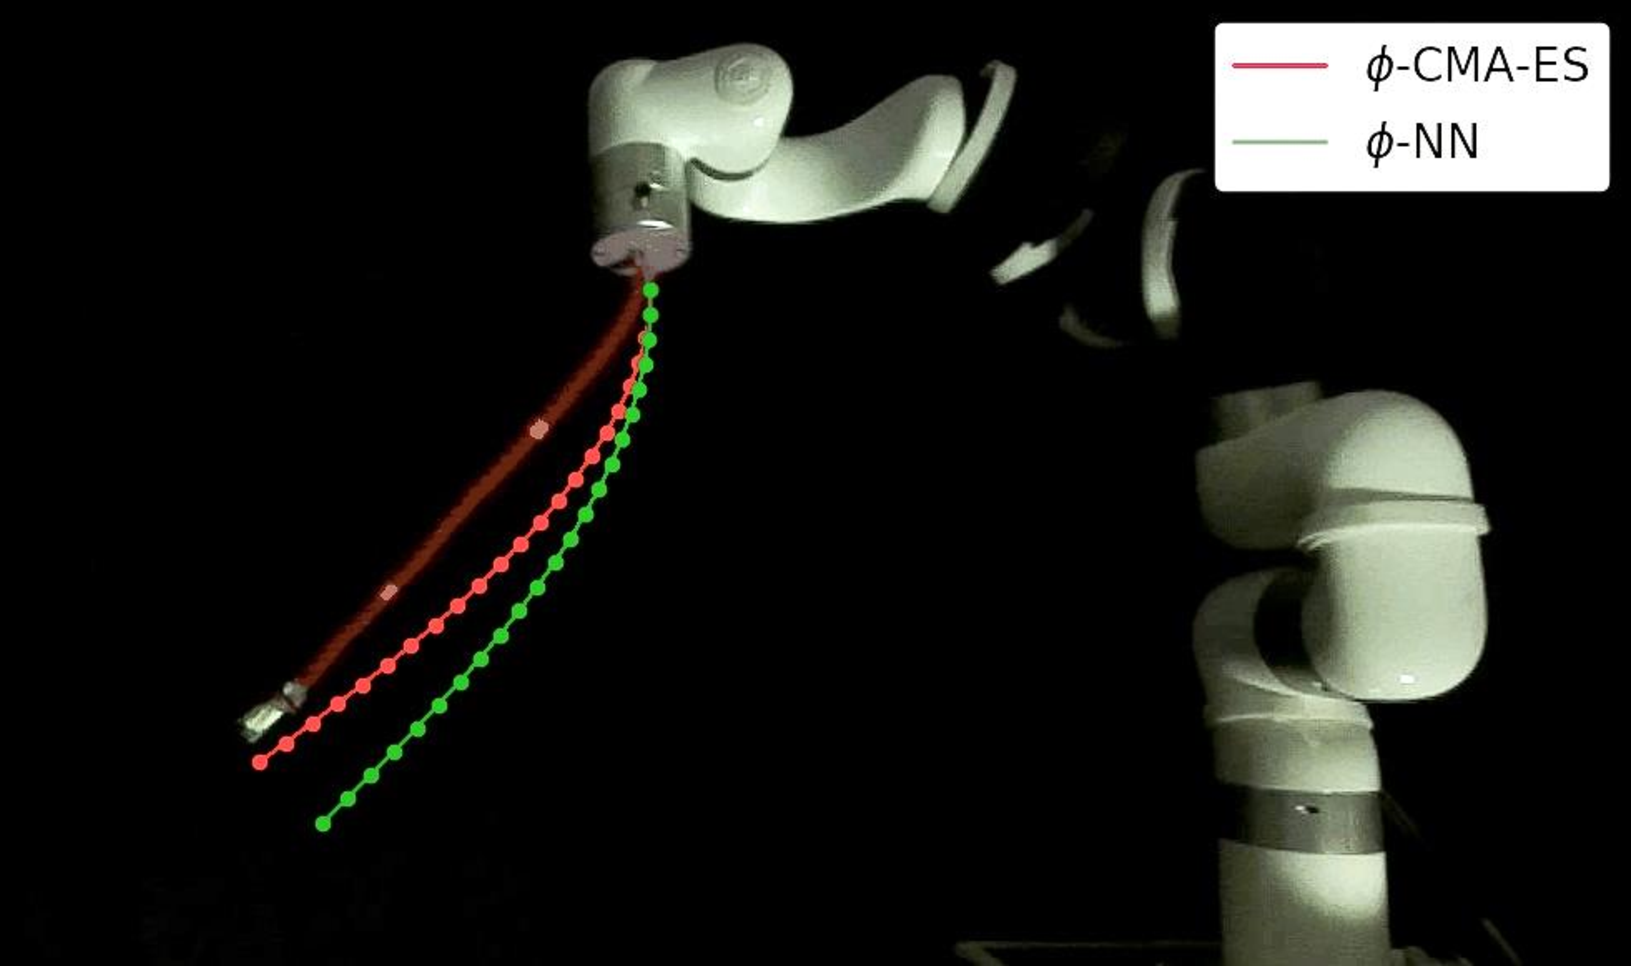
\includegraphics[width=0.8\columnwidth]{images/overlay_sim_to_robot.pdf}
    \caption{Real and simulation comparison for $\Phi$-NN benchmarking and $\Phi$-CMA-ES on an unseen dynamic motion.}
    \label{fig:pointwise-comparison}
\end{figure}

\begin{figure} 
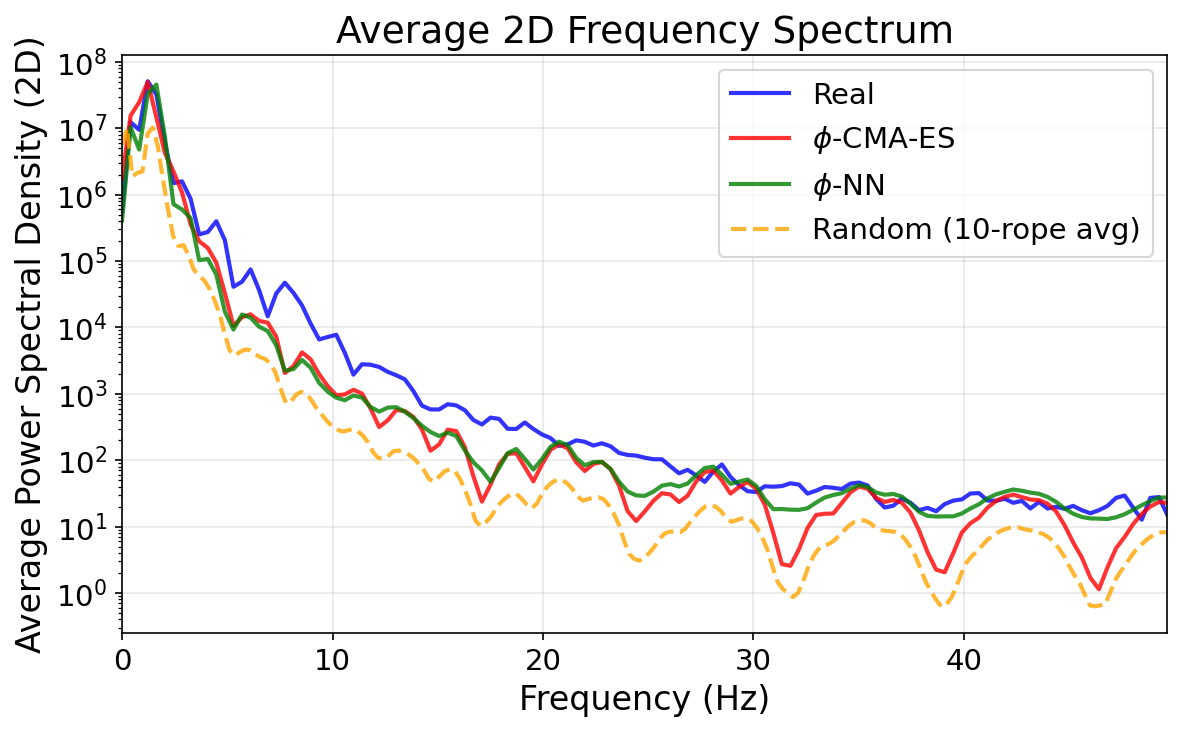
\includegraphics[width=0.92\columnwidth]{images/fourier_good_text_size.png}
\caption{Fourier frequency distributions on the Red (45\,cm, 10g lead) rope with simulated predictions from $\Phi$-CMA-ES and $\Phi$-NN on a test set motion. Appendix tab. 1; similar trends can be seen across ropes.}\label{fig:fourier}
\end{figure}

\textbf{Task-Level Validation.} We first validate in simulation that predicted parameters enable downstream trajectory optimization. For 100 random simulated ropes, we predict parameters with $\Phi$-NN, optimize trajectories using those predictions (CMA-ES-traj, Section~\ref{sec:cmaes-traj}), and measure task error (Table~\ref{tab:sim-full}). Trajectories optimized with predicted parameters achieve 2.1\,cm median error versus 1.2\,cm with ground truth and 12.8\,cm with random in-distribution parameters. Predicted parameters provide 6$\times$ improvement over uninformed baselines while remaining within 0.9\,cm of ground truth performance. This demonstrates that parameter estimation errors do not compound catastrophically, suggesting $\Phi$-NN provides sufficient information for control, validating the two-stage pipeline design.

\textbf{Parameter Importance.}
\label{sec:param_importance}
The preceding results show that $\Phi$-NN's predictions are collectively sufficient for successful task rollout, but do not reveal which of the nine parameters actually drive that success. We study this in two complementary ways, both in simulation.

We first run a single fixed robot trajectory while varying each of the nine parameters independently across its training range, holding the others fixed. For every parameter, the resulting tip-position variance exceeds \SI{5}{cm} at many points along the trajectory: no parameter can be safely ignored, each contributes measurably to the rope's dynamic response under an identical action.

We then quantify how task accuracy degrades when subsets of $\Phi$-NN's predictions are replaced with random in-distribution values. For each of 30 rope configurations drawn from our real-world evaluation, we generate 10 random-parameter sets per configuration and evaluate 3D pole-striking accuracy in simulation under five conditions (Table~\ref{tab:param_importance}). Retaining only the length and lead-mass predictions, the two parameters one might expect to dominate, while randomizing the remaining seven still yields mean error above \SI{10}{cm}. Length and lead mass are among the easiest to identify by the neural network, but approximately accurate estimates of the remaining seven are also required for accurate trajectories. 

\begin{table}[h]
\centering
\small
\setlength{\tabcolsep}{4pt}
\renewcommand{\arraystretch}{0.95}
\caption{Parameter importance ablation. Each row replaces a subset of $\Phi$-NN's nine predictions with random in-distribution values, keeping $\Phi$-NN's predictions only for the parameters listed. Evaluated in simulation over 10 random parameter sets per each of 30 rope configurations from our real-world evaluation.}
\label{tab:param_importance}
\begin{tabular}{l
    S[table-format=2.1]
    S[table-format=2.1]}
\toprule
\textbf{Condition (simulation)} & \textbf{Mean (\si{cm})} & \textbf{Std (\si{cm})} \\
\midrule
$\Phi$-NN (full pipeline)                 & 0.9  & 0.4  \\
Random + $\Phi$-NN length \& lead mass    & 10.9 & 10.1 \\
Random + $\Phi$-NN length only            & 13.3 & 13.5 \\
Random + $\Phi$-NN lead mass only         & 12.3 & 10.5 \\
Fully random in-distribution              & 14.2 & 12.5 \\
\bottomrule
\end{tabular}
\end{table}

\subsection{Action Policy Optimization Evaluation} \label{sec:cma-es-traj-eval}

The trajectory returned by CMA-ES ~\ref{sec:cmaes_traj} consistently converges to a solution for all of our tasks when given 25 iterations for 3D Point Striking ($\sim$25 minutes), 50 iterations for lobbing ($\sim$120 minutes) and 15 iterations for draping ($\sim$60 minutes). For 3D point striking, the trajectory returned by CMA-ES found actions that resulted in an average rope tip distance of 0.8\,cm from the goal position. We observe that with a dt in simulation of 0.01, and the high speeds of rope manipulation tasks, the ground-truth moment of minimum distance is often missed by a small margin likely meaning the method is achieving even lower true accuracy than our reported averages. For other tasks, CMA-ES was consistently able to find solutions, although we did find that without the correct reward and penalty structure, CMA-ES-traj often would push the limitations of the stability of Drake. 

\begin{table}[t]
\centering
\caption{Average of 100 adaptation-predicted ropes on full pipeline in simulation. Comparison of ground truth, predicted and 100 random in-distribution ropes. Here, CMA-ES-traj was optimized until 25 iterations \textit{or} min-distance of $<$1.5cm}
\label{tab:sim-full}
\begin{tabular}{
    l 
    S[table-format=2.1] 
    S[table-format=1.2] 
    S[table-format=3.1] 
    S[table-format=2.1]
    @{\,${}\pm{}$\,}
    S[table-format=2.1]
}
\toprule
 & {\textbf{Median}} & {\textbf{Min}} & {\textbf{Max}} & \multicolumn{2}{c}{\textbf{Mean}} \\
\midrule
\textbf{Ground Truth} & 1.2 & 0.25 & 21.6 & 1.4 & 2.2 \\
\textbf{Predicted} & 2.1 & 0.27 & 70.2 & 5.7 & 11.5 \\
\textbf{100 random ropes} & 12.8 & 0.14 & 104.3 & 16.3 & 12.1 \\
\bottomrule
\end{tabular}
\end{table}

\subsection{Full Pipeline Results in Real} \label{sec:fullpipeline}

We test on four in-domain ropes with a diverse range of system attributes as shown in Fig. \ref{fig:ropes} and described in Table \ref{tab:rope_descriptions} and one out-of-domain metal chain to understand the generalizability of our model. For each rope we tested a 45\,cm, 55\,cm, and 65\,cm version (each with a 5\,g lead attached). We also tested each 45\,cm rope with 10\,g, 20\,g, and 30\,g leads. The per-parameter breakdown is included in Table \ref{tab:rope_results}. We observe a similar trend as we did in simulation, wherein both $\Phi$-NN and $\Phi$-CMA-ES demonstrate useful system parameter outputs for task optimization. $\Phi$-CMA-ES, a na\"ive system adaptation through overfitting, serves as a useful benchmark to see how $\Phi$-NN performs. We observe that our method outperforms $\Phi$-CMA-ES on average for in-distribution models. It is expected that for out-of-distribution ropes, $\Phi$-CMA-ES would find a more suitable representation to explicitly match the rope. We use $\Phi$-Random to benchmark the impact of system parameters for task optimization and to demonstrate that the CMA-ES action trajectories are not producing one-action-fits-all ropes. $\Phi$ Random represents a set of 20 in-distribution ropes for which we optimized a trajectory and executed the optimized trajectory on our test ropes. This simulates what would happen if our system-identification were drastically incorrect or not performed, but the action was still educated (i.e. there is a rope with which this action would be optimal). We did not perform $\Phi$-Random tests on the chain for safety. Our test suggest that personalized parameters from $\Phi$-NN for each rope results in a four times accuracy improvement compared to the non-system-identified trials. We note, for our experiments when the pole was directly hit, the instantaneous velocity change made distance estimations incorrect; if the lead was on target (hitting the correct black tape in Fig.~\ref{fig:system_overview}) we marked a \textit{0.00} distance.


\begin{table}[t]
\footnotesize
\centering
\caption{Full pipeline results after rope wiggle, parameter prediction, CMA-ES-traj execution. Average distance (cm) from target reported from 600 task-policy rollouts (5 per).}
\label{tab:rope_results}
\begin{threeparttable}
\begin{tabular}{@{}l@{\;}c@{\;}c@{\;}c@{\,}c@{\,}c@{\,}c@{\,}c@{\,}c@{}}
\toprule
\multirow{3}{*}{\textbf{Rope}} & \multirow{3}{*}{\textbf{Method}} & \multicolumn{6}{@{}c@{}}{\textbf{Length and Lead Weight}} & \multirow{3}{*}{\textbf{Avg}} \\
\cmidrule(lr){3-8}
& & \textit{45cm} & \textit{45cm} & \textit{45cm} & \textit{45cm} & \textit{55cm} & \textit{65cm} & \\
& & \textit{5g} & \textit{10g} & \textit{20g} & \textit{30g} & \textit{5g} & \textit{5g} & \\
\midrule
\multirow{3}{*}{\textcolor{Brown}{Brown}} 
& $\Phi$-NN & 0.14 & 2.03 & \textbf{5.28} & \textbf{0.82} & \textbf{0.00} & \textbf{2.07} & \textbf{1.72} \\
& $\Phi$-CMA-ES & \textbf{0.00} & \textbf{0.61} & 8.86 & 5.24 & 0.20 & 4.43 & 3.22 \\
& $\Phi$-Random & 15.88 & 17.34 & 18.28 & 17.70 & 15.47 & 22.14 & 17.80 \\
\midrule
\multirow{3}{*}{\textcolor{Dandelion}{Yellow}} 
& $\Phi$-NN & 8.11 & 6.27 & 0.78 & 4.71 & \textbf{3.47} & \textbf{0.00} & \textbf{3.89} \\
& $\Phi$-CMA-ES & \textbf{1.47} & \textbf{3.76} & \textbf{0.76} & \textbf{3.25} & 7.69 & 8.07 & 4.17 \\
& $\Phi$-Random & 14.65 & 15.85 & 16.50 & 16.97 & 14.98 & 19.25 & 16.37 \\
\midrule
\multirow{3}{*}{\textcolor{Red}{Red}} 
& $\Phi$-NN & \textbf{0.00} & 15.96 & \textbf{0.91} & \textbf{1.37} & \textbf{0.33} & 4.27 & 3.81 \\
& $\Phi$-CMA-ES & \textbf{0.00} & \textbf{3.19} & 2.34 & 7.18 & 1.39 & \textbf{0.00} & \textbf{2.35} \\
& $\Phi$-Random & 17.63 & 15.23 & 16.95 & 16.59 & 14.05 & 18.17 & 16.44 \\
\midrule
\multirow{3}{*}{\textcolor{Orange}{Orange}} 
& $\Phi$-NN & 10.08 & \textbf{2.16} & 3.71 & \textbf{0.00} & 11.45 & \textbf{1.33} & \textbf{4.79} \\
& $\Phi$-CMA-ES & \textbf{0.00} & 8.65 & \textbf{1.50} & \textbf{0.00} & 12.04 & 19.06 & 6.88 \\
& $\Phi$-Random & 10.90 & 9.99 & 11.82 & 13.51 & 8.00 & 9.06 & 10.55 \\
\midrule
\multirow{2}{*}{\textcolor{CadetBlue}{Chain*}} 
& $\Phi$-NN & 51.37 & 29.60 & 12.33 & 3.31 & 51.94 & \textbf{0.69} & 24.87 \\
& $\Phi$-CMA-ES & \textbf{3.86} & \textbf{0.63} & \textbf{2.65} & \textbf{1.55} & \textbf{4.46} & 6.68 & \textbf{3.30} \\
\midrule
\multicolumn{2}{@{}l@{}}{\textbf{Avg In-Domain ($\Phi$-NN)}} & 4.58 & 6.61 & \textbf{2.67} & \textbf{1.73} & \textbf{3.81} & \textbf{1.92} & \textbf{3.55} \\
\multicolumn{2}{@{}l@{}}{\textbf{Avg In-Domain ($\Phi$-CMA-ES)}} & \textbf{0.37} & \textbf{4.05} & 3.37 & 3.92 & 5.33 & 7.89 & 4.16 \\
\bottomrule
\end{tabular}
\begin{tablenotes}
    \item * out-of-domain
\end{tablenotes}
\end{threeparttable}
\end{table}


\subsubsection{Secondary Tasks: Lobbing and Draping}

We include our in-real results from our secondary tasks in Table~\ref{tab:combined_tasks}. These examples demonstrate the ability of our pipeline to perform actions with more complex reward structures with system identification information as a strong prior. We use two metrics to assess success for both methods due to the multi-objective reward function. For lobbing, we consider it a full success if the rope tip both knocks a domino down and remains on the board (demonstrating a gentle lob onto the surface). We place the domino closer to the simulation robot to reflect that to knock an object over both humans and robots must estimate to overshoot striking the object. For the task of draping we judge a successful drape if it hangs over the wall (i.e. tip is over the wall and hanging) and secondary success is judged by the distance of the midpoint of the rope to the top of the wall which was used directly as a metric for CMA-ES-traj's reward function for this task. These additional experiments validate the theoretical construction of a task corpus $\mathcal{T}$ which consists of system-parameter informed models which are all informed by $\Phi$.
Because $\Phi$ is shared across the corpus, incorporating a new task requires only a representative simulation environment and a reward function, with no retraining of the identification module.

\begin{table}[t]
\centering
\caption{Performance across lobbing and draping tasks with different parameter prediction methods.}
\label{tab:combined_tasks}
\begin{threeparttable}
\begin{tabular}{@{}ll@{\hspace{1pt}}c@{\hspace{3pt}}c@{\hspace{8pt}}c@{\hspace{3pt}}c@{}}
\toprule
& & \multicolumn{2}{c@{\hspace{8pt}}}{\textbf{Lobbing}} & \multicolumn{2}{c}{\textbf{Draping}} \\
\cmidrule(lr){3-4} \cmidrule(l){5-6}
\textbf{Rope} & \textbf{Method} & \textbf{Target} & \textbf{Stay} & \textbf{Success} & \textbf{Distance (cm)} \\
\midrule
\multirow{2}{*}{\textcolor{Brown}{Brown}} 
 & $\Phi$-NN & 67\% & 50\% & 67\% & 4.1 \\
 & $\Phi$-CMA-ES & 83\% & 33\% & 83\% & 3.8 \\
\addlinespace
\multirow{2}{*}{\textcolor{Dandelion}{Yellow}} 
 & $\Phi$-NN & 67\% & 17\% & 67\% & 7.4 \\
 & $\Phi$-CMA-ES & 67\% & 50\% & 67\% & 4.1 \\
\addlinespace
\multirow{2}{*}{\textcolor{Red}{Red}} 
 & $\Phi$-NN & 67\% & 17\% & 67\% & 3.6 \\
 & $\Phi$-CMA-ES & 83\% & 50\% & 67\% & 4.8 \\
\addlinespace
\multirow{2}{*}{\textcolor{Orange}{Orange}} 
 & $\Phi$-NN & 17\% & 0\% & 50\% & 3.4 \\
 & $\Phi$-CMA-ES & 17\% & 17\% & 50\% & 3.5 \\
\midrule
\multicolumn{2}{l}{\textbf{Avg In-Domain ($\Phi$-NN)}} & 54\% & 21\% & 63\% & 4.6 \\
\multicolumn{2}{l}{\textbf{Avg In-Domain ($\Phi$-CMA-ES)}} & 63\% & 38\% & 67\% & 4.1 \\
\bottomrule
\end{tabular}
\begin{tablenotes}
\small
\item Averages for 6 configurations per rope; full results in appendix
\end{tablenotes}
\end{threeparttable}
\end{table}


\section{Limitations}
\label{sec:limitations}
 
CMA-ES-traj under Drake is CPU-bound, capping per-task throughput at 25--120 minutes depending on task and environment complexity (Sec.~\ref{sec:cma-es-traj-eval}); as discussed in Sec.~\ref{sec:cmaes-traj}, $\Phi$-NN's task-agnostic output is theoretically compatible with any future GPU-accelerated or gradient-based optimizer. We think using reinforcement learning for trajectory policy learning is an exciting future direction. $\Phi$-NN's predictions saturate at the bounds of its training distribution (Sec.~\ref{sec:wiggleablation}), and because all nine parameters contribute to downstream accuracy (Sec.~\ref{sec:param_importance}), saturation on any single dimension degrades the whole prediction. 

One limitation of our work is that there was a large amount of noise in segmentation and tracking in the real-to-sim transfer. Our current simulation environments have some limited capabilities to accurately represent real rope behavior such as kinks. 
 
\section{Conclusion and Future Work}
 
This paper introduces a novel, task-agnostic system identification method for rope manipulation. Through the use of a single safe action and the leveraging of simulation priors with a neural network model we can fit descriptive system parameters to a rope in real. On 3D pole-striking this yields roughly a four-fold improvement in real-world accuracy over non-system-identified baselines, and the same identification module extends without modification to lobbing and draping.
 
We believe there are many exciting future possibilities to fine-tune the system-identification accuracy. We hypothesize there exist wiggles that can excite the rope in a more targeted manner to isolate individual system parameters.

\bibliographystyle{plainnat}
\bibliography{references}
\clearpage
\input supp

\end{document}